\section{Further Experiments}
\subsection{Additional Features}
We tested out several other features, but discarded them later as they did not improve results. They were: 
\begin{enumerate}
\itemsep0em 
\item Number of connected holes.
\item Difference between maximum and minimum column height.
\item Maximum depth of well. 
\item Number of blocks currently present on the board.
\item Weighted number of blocks, where you penalize blocks in proportion to the height at which it is located.
\item Number of Horizontal transitions.
\item Number of Vertical transitions.
\end{enumerate}

\subsection{Other heuristics for crossing over}
We experimented with some other heuristics for performing the crossing over of the two parents to generate the child :
\begin{enumerate}
\itemsep0em 
\item The child randomly picks the full set of weights of one of its parents 
\item The child's weights are average of weights of the parents
\item For each feature, the child randomly inherits the weight from one of the parents
\item Generate a random number k, and the child takes the first k weights from one parent and the rest from the other
\end{enumerate}
However, we got a maximum of 86,516 cleared rows with these other heuristics and thus discarded them. Graphs for analyzing performance of these heuristics can be found in the appendix.


% \subsubsection{Alternative Training Algorithm}
%  We experimented with the method for performing the crossing over.
% \newline
% To formulate a new generation, 30\% of the best performing parents from the previous generation are directly passed as children, while the remaining 70\% of the population is generated as follows :
% \newline
% Randomly a subset (25\%) of members from the previous generation is chosen. Then from this subset the member with best performing set of weights is chosen as the first parent. The other parent is picked from a different subset, using the same approach. 
% \newline
% After the parents have been selected, a heuristic defines how to perform the crossing over, i.e. how the child evolves from its parents. During the project, there were several heuristics that we tested: 


% We also designed a fitness function which checks if the newly generated child performs as least as good as the worst child so far in the population. If this isn't the case, it is replaced by a newly generated child that results from another crossing-over process. To avoid infinite loops, an upper limit for the number of children which can be rejected is fixed to 5. 

\subsection{Particle Swarm Optimization (PSO)}
PSO is a computational method that iteratively tries to improve a candidate solution with respect to a given measure of quality. At each iteration, it keeps track of the best feature weights for every population member, and also for the entire population. We modify the weights at each iteration, influenced by the best weights for that member as well as for the entire population, using the velocity vector for each feature, and update them in case a personal best or global best set of weights is found(which clears the most number of rows). This optimization directs the movement of weights of the future generations based on memory of best performing members of the previous generations. This helps converge the current genetic agent candidate towards the most optimal one found so far.

\subsection{Other Algorithms}
Using a genetic algorithm is capable of finding a well-performing solution but still heavily depends on the features engineered by humans. Thus, we tested data-driven algorithms in order to eliminate the necessity of human feature engineering.  

\subsubsection{Q Learning}
Q Learning is a kind of reinforcement learning, that does not require a model of its environment. For each game state ($s$), Q Learning maps all possible actions ($a$) to rewards $Q(s,a) $. The Q function's values for each pair $(s,a)$ is derived during training procedure, using the Bellman equation \cite{qlearning}: 

$$Q(s,a) = r + \gamma \max_{a'} Q(s', a')$$

Meaningly, the reward for taking action $a$ in state $s$ is the sum of the initial reward of this action $(r)$ and the weighted reward of the next state $s'$. In order to get a Q value for all actions in every state, during training time, a random action is chosen with probability $\epsilon = 0.4$. Otherwise, the greedy policy determines the action. The training is terminated when all of the Q-values converged. This might include to have a decreasing learning and random move picking rate ($\gamma$ resp. $\epsilon$). 
\newline
The Q-learning approach is therefore in need of a reward function (r) but in contrast to the genetic algorithm approach this is very intuitive e.g. for Tetris, $r=-1$ if the game has ended and $r=0$ otherwise is sufficient, or for CTB, $r=1$ if the ball was cought and $r=-1$ if the ball passed the catcher (see chapter \ref{sec:generality}). 

\vspace{0.25cm}

Therefore the Q learning method is capable of playing any game without any a priori knowledge about the environment, only terminal state games have to be assigned a "reward". Nevertheless a lot of training iterations are necessary until all of the Q values converged and have been updated at least once. While this does not pose a problem in case of small states and action spaces, as in the CTB game with $\mathcal{O}(10^2)$ possible pairs, indeed the Q learning training procedure is infeasible in case of large state spaces. The Tetris as characterized in \ref{sec:problem} has $2^{200} = \mathcal{O}(10^{60})$ states. Even if one training iteration would take less than a nanosecond and the algorithm would never revisit states updating every entry in the Q matrix would require roughly $10^{43}$ years. It can nevertheless be shown that the Q learning approach works in the Tetris frame. For a simpler version of Tetris \footnote{The simpler Tetris game differs from the "standard" Tetris game in matters of both the board size (3x3) and the set of Tetraminos (2) used, in order to reduce the space-action-space.} the Q values converged after 10000 iterations and afterwards the agent clears an infinite number of rows. Thus, to solve the "standard" Tetris game with a Q-Learning approach, the challenge is to narrow the state space dramatically and reasonably. 

\vspace{0.25cm}

For the purpose of shrinking the state-space several approaches were tested. Most of our approaches resulted in a too large loss of information and consequently to a very bad performance of the agent (e.g. redefining the game's state as the top (two) rows of the board). 

\subsubsection{Auto Encoder}
High-dimensional data can be converted to a lower-dimensional representation by training a multilayer neural network. This network (see figure \ref{fig:encoder_arch}) is symmetric with respect to the small central layer (whose output is the encoded input). Therefore the first part of the network encodes the data, while the second one decodes it and the resulting error is used to optimize the networks' weights (\cite{autoencoder}). In the Tetris game an auto encoder can be used to encode the field (state) and replace it by a low-dimensional column vector. 

\begin{Figure}
\centering
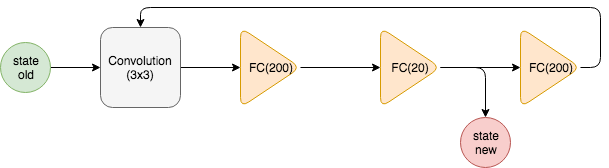
\includegraphics[width=8cm]{imgs/encoder_structure.png}
\captionof{figure}{Auto Encoder - Architecture}
\label{fig:encoder_arch}
\end{Figure}

To represent the Tetris board in a lower-dimensional space the adjacent structure of every cell (e.g. holes) could be important. Hence, the board is convoluted first and the convoluted board is fed into the autoencoder which consists of three fully connected layers, down-sampling to a vector of size 20, and is trained using batch-normalized stochastic gradient and subsequently steepest gradient descent, to avoid getting stuck in a local minimum (compare \ref{fig:encoder_errors}). For building and training the network the encog framework \cite{encog} was deployed.

\subsubsection*{Auto Encoder in Genetic Algorithm}
Instead of manual feature engineering the features could be derived by learning a shrunk state representation, i.e. by using the auto encoder's state directly. We used our CTB implementation to first verify this new general idea. To perfectly perform in the CTB game (section \ref{sec:appendix}) merely the distance between catcher and ball is necessary as a state, a full state description is given by the distance and a position of either the catcher or the ball (merely x-coordinate regarded here). In theory the game's internal state, i.e. two hot-encoded vectors containing the discrete x-position of both catcher and ball, should be down-sampled to this smallest possible state description. Unfortunately, applying an autoencoder to the CTB game results in two values that are not separately dependent on either the distance or position but contain a combination of both. Thus, even if the encoder's output well defines the game's state, it can nevertheless not be used as feature vector, since the agent's decision should surely not be affected by the absolute position of catcher/ball in the CTB example. In general the previously described problem arises as well when applied on the Tetris game. Hence, the genetic agent trained with autoencoded features did not perform well for the two games.

\section{General Agent}
\label{sec:generality}
Another goal of our project was to design the agents in a general style such that they are not limited to only playing Tetris, but can be easily deployed and tested on CTB or any other game which is implemented in line with our abstract (general) game class. The roadbloack here is that we have not yet found an algorithm which can automatically calculate reasonable set of features. Therefore human "feature engineering" will still be required. 

\begin{Figure}
\centering
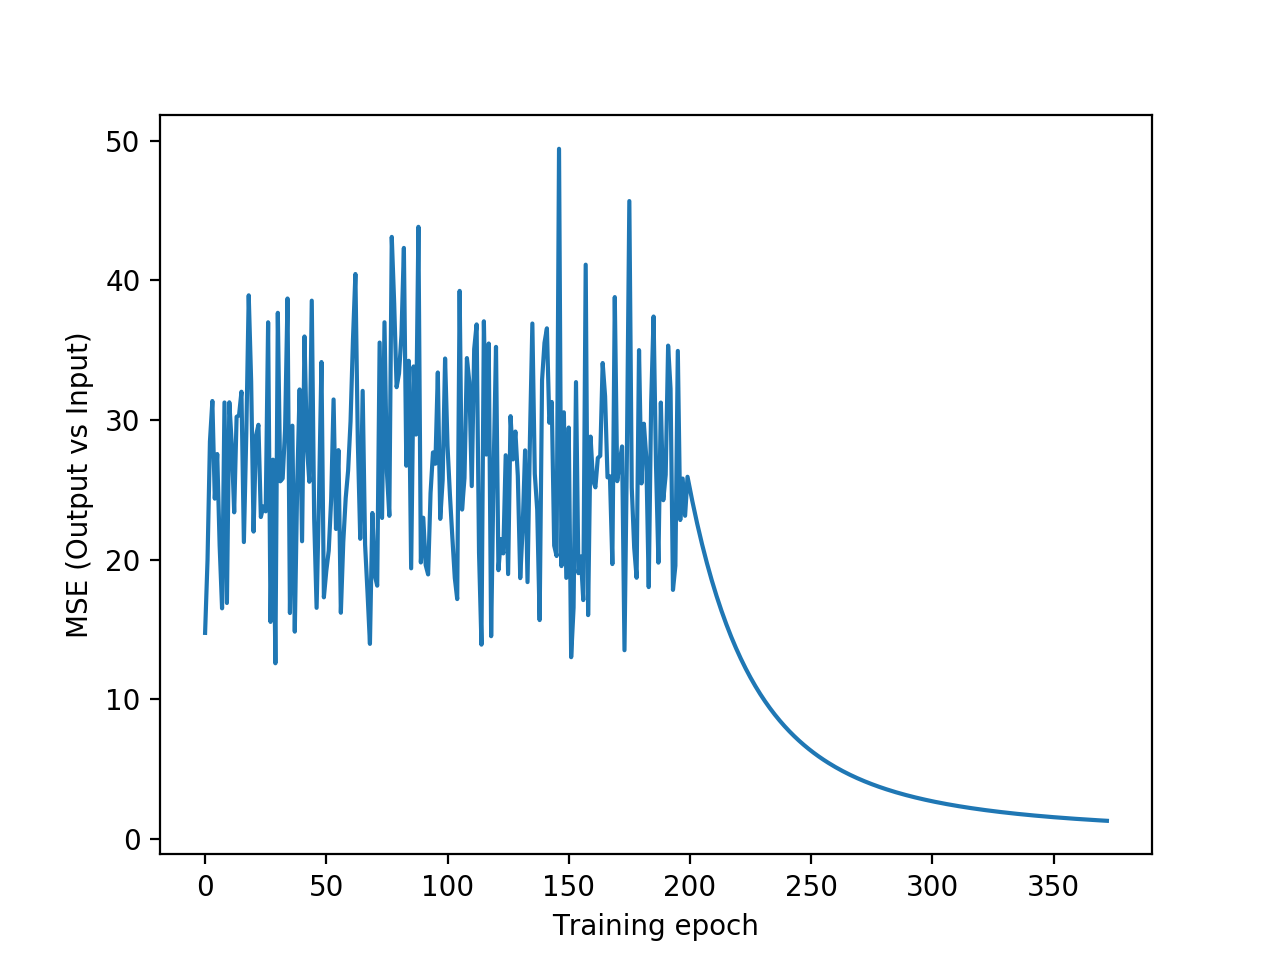
\includegraphics[width=6cm]{imgs/encoder_errors.png}
\captionof{figure}{Auto Encoder - Training errors}
\label{fig:encoder_errors}
\end{Figure}

% \subsubsection*{Auto Encoder - Q Learning}
% Although the auto encoder described above manages to down-sample the state-space dramatically its output is not discrete, as required for the Q learning approach. In order to apply a Q learning based approach deep Q learning would have to be used, which is behind the scope of this project.

  
